\begin{flushleft}
{\Huge Djungelvrål\\}
{\Large
\vspace{1cm}
Ute i skogen är det mörkt, kallt och läskigt. Om man blir rädd eller
bara är lite orolig finns det inget bättre än att samstämt lätta på
rädslan i glad sång. Skuggorna bakom träden försvinner, humöret växer
och lägerelden värmer än bättre. Om ni är på hajk, på svamputflykten eller på
orienteringsrundan kan ni med fördel sjunga dessa sånger.}
   
\end{flushleft}
\vspace{2cm}
\begin{center}
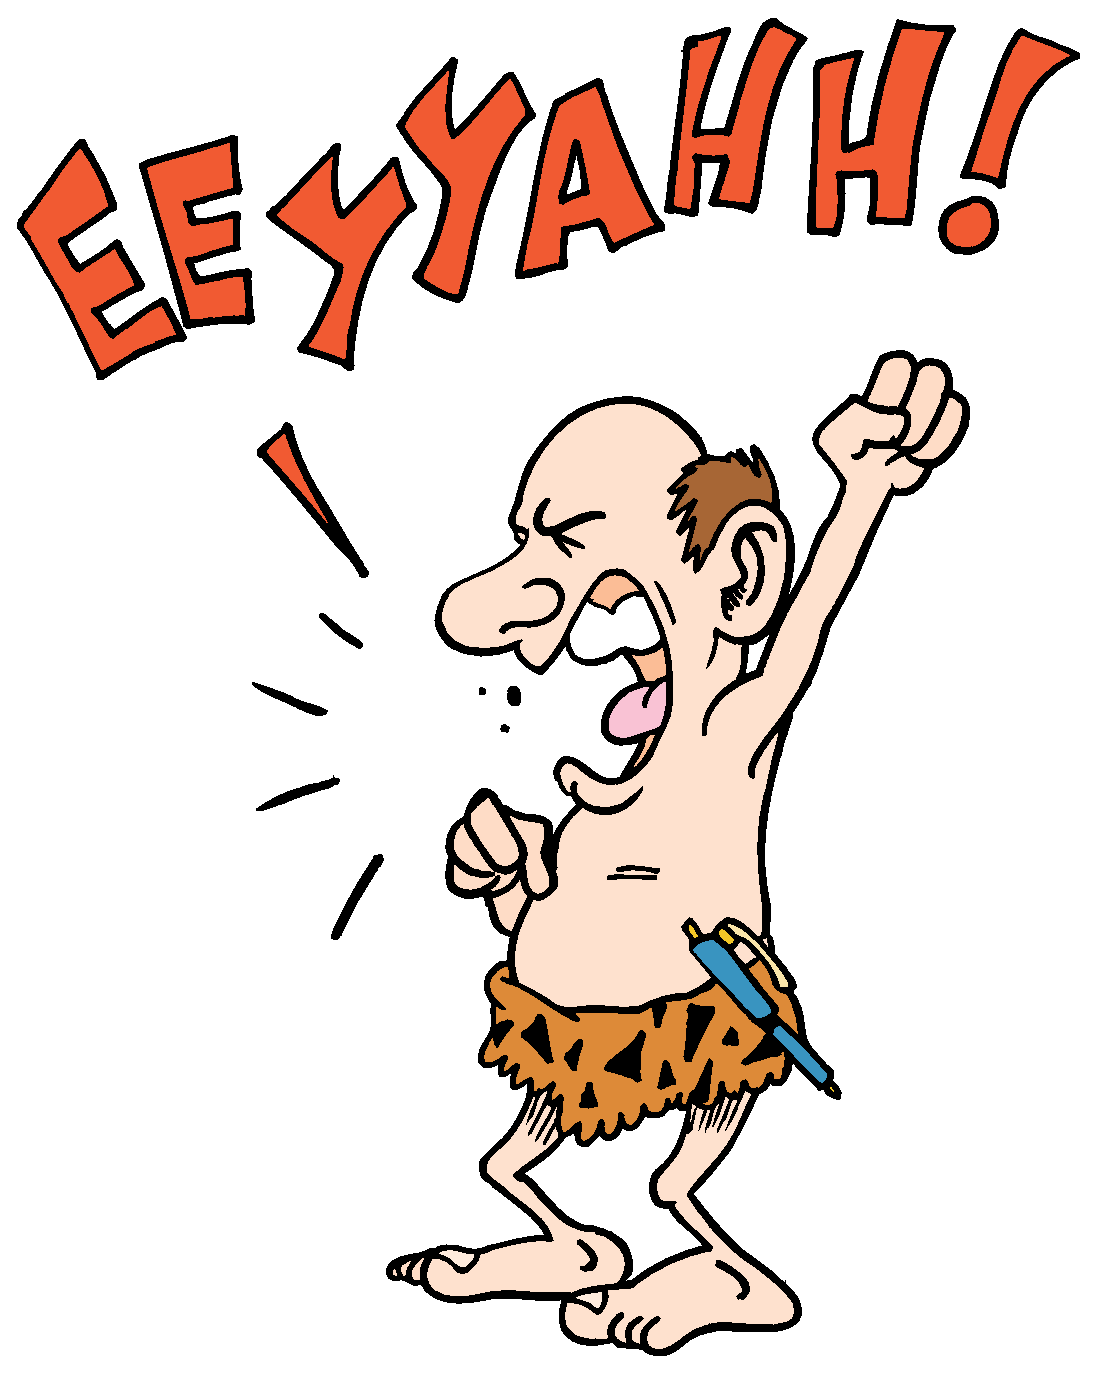
\includegraphics[width=6cm]{bilder/120.eps}

\end{center}
 

\newpage
\begin{song}{ABC}{abc}
\begin{vers}
Timmen är slagen nu slutar vi för dagen,\\
går hem till mig, jag skall förhöra dig.\\
\end{vers}
\begin{vers}
ABC, du är i mina tankar\\
CDE, mitt hjärta det bankar,\\
EFG, du får mig alltför lätt ur balans.\\
ABC, du är i mina tankar\\
CDE, mitt hjärta det bankar,\\
EFG, du ger mig ingen ärlig chans.\\
\end{vers}
\begin{vers}
Du är den bästa i hela klassen, i biologi.\\
Du läser på till och med på rasten om kärlekens kemi.\\
Du är inte som alla andra.\\
Du är min första kärlek.\\
Du är alla tjejernas dröm.\\
Matematik, tillsammans är vi två.\\
Som ljuv musik, do re mi fa so la-a-a-a.\\
\end{vers}
\begin{vers}
ABC, du är i mina tankar\\
CDE, mitt hjärta det bankar,\\
EFG, du ger mig ingen ärlig chans.\\
\end{vers}
\begin{vers}
Jag känner nånting, ja det händer nånting,\\
det är nånting som brinner i mig.\\
Kärleken vaknar, å vad jag saknar,\\
känslan att hålla i dig.\\
Biologi, är kärlekens magi.\\
Min melodi, ikväll så är jag fri-i-i-i-i.\\
\end{vers}
\begin{vers}
ABC, du är i mina tankar\\
CDE, mitt hjärta det bankar,\\
EFG, du får mig alltför lätt ur balans.\\
ABC, du är i mina tankar\\
CDE, mitt hjärta det bankar,\\
EFG, du ger mig ingen ärlig chans.\\
ABC, du ger mig ingen ärlig chans.\\
\end{vers}
\end{song}

\begin{song}{The lion sleeps tonight}{thelion}
\begin{vers}
In the jungle, the mighty jungle, \\
the lion sleeps tonight.\\
In the jungle, the mighty jungle, \\
the lion sleeps tonight.\\
Wee-ooh wim-o-weh.\\
//: Wim-o-weh o-wim-o-weh o-wim-o-weh o-wim-o-weh\\
o-wim-o-weh o-wim-o-weh o-wim-weh. ://\\
\end{vers}
\begin{vers}
Near the village, the peaceful village, \\
the lion sleeps tonight.\\
Near the village, the peaceful village, \\
the lion sleeps tonight.\\
Wee-ooh wim-o-weh...\\
Hush, my darling, don't fear, my darling, \\
the lion sleeps tonight.\\
Hush, my darling, don't fear, my darling, \\
the lion sleeps tonight.\\
Wee-ooh wim-o-weh...\\
\end{vers}
\end{song}

\newpage

\begin{song}{Fantomens brallor}{fantomensbrallor}
\begin{vers}
Ingen har sett Fantomen utan kläder\\
klädd i pyjamas och stövlar av läder.\\
Han drar nog bort en rand där fram\\
när han kissar bakom trädets stam.\\
\end{vers}
\begin{vers}
Refr:\\
O, vandrande vålnad, kliar inte sviden\\
när du knegar i djungeln hela tiden?\\
Gör som Guran, skaffa dig en kjol,\\
det är bättre under Afrikas sol.\\
\end{vers}
\begin{vers}
Ingen har sett honom kavla upp ärmen\\
ljusblå lekdräkt i fukten och värmen.\\
Men han blev nog frusen om sin häck\\
Om han satt i grottan alldeles näck.\\
\end{vers}
\begin{vers}
Refr\\
\end{vers}
\begin{vers}
Fantomen lättar inte på kalsongen\\
nej, han håller värmen stången.\\
Ibland tar han på sig ännu mer\\
när Mr Walker sig till staden beger.\\
\end{vers}
\begin{vers}
Refr\\
\end{vers}
\end{song}

\newpage

\begin{song}{Kung Louis sång}{kingloui}
\begin{vers}
Jag kungen är över alla här\\
under trädens gröna höjd.\\
Jag har nått opp, till högsta topp,\\
men ännu är jag ej nöjd.\\
Jag vill ju va en man, en mänska, \\
och kunna allt Ni kan.\\
Jag vill inte längre apa mig, \\
jag vill ju bara va en man.\\
\end{vers}
\begin{vers}
Refr:\\
Oh, obido. Jag vill va som du.\\
Jag vill se ut som du, gå som du-u-u.\\
Det vill jag nu, ett djur som jag. (ubi dubi dubi)\\
Det lär sig bra bli en människa.\\
\end{vers}
\begin{vers}
Försök inte lura mig gosse, \\
jag inga konster tål.\\
Att känna till hur eld blir till, \\
det är mina drömmars mål.\\
Din hemlighet vill jag veta, \\
seså säg hur det går till.\\
För då blir jag visst, en man till sist, \\
och det är ju vad jag vill.\\
\end{vers}
\begin{vers}
Refr\\
\end{vers}
\end{song}

\begin{song}{Var nöjd med allt som livet ger}{varnojd}
\begin{vers}
Var nöjd med allt som livet ger \\
och allting som du kring dig ser,\\
glöm bort bekymmer, sorger och besvär. \\
Var glad och nöjd, för vet du vad? \\
En björntjänst gör ju ingen glad.\\
Var nöjd med livet som vi lever här. \\
Varthän jag än strövar, varthän jag än går \\
står ljung och snår kring mina spår. \\
Jag älskar bin och deras bon, \\
för honung är ju min passion\\
och vill du av myror ha munnen full \\
så ta en titt under sten och mull.\\
- Äta myror?\\
- Ha, ha, det är världens käk.\\
Kittlar dödsskönt i kistan. \\
Var nöjd med allt du ser och allt som livet ger.\\
Var nöjd...\\
Om frukter dig lockar, banan eller bär.\\
Se till att du plockar dem utan besvär. \\
Vill du plocka frukt av bästa klass \\
så använd din höger och vänster tass, \\
men klorna dom skall du dra in\\
så fort du ska ta dig en fin apelsin.\\
- Hoppas att du har förstått?\\
- O, ja! Tack Baloo!\\
Var nöjd...\\
\end{vers}
\end{song}


\begin{song}{Patrullmans sång}{patrullmanssang}
\mel{House of the Rising Sun}
\begin{vers}
Jag har ett glas uti min hand\\
till brädden fyllt med sprit.\\
Jag tar mig så en tår på tand,\\
en Skåne Akvavit.\\
\end{vers}
\begin{vers}
Patrullman, broder, om du vill,\\
drick ur tills du blir nöjd.\\
Skåla sedan alla till\\
i gamman och i fröjd.\\
\end{vers}
\end{song}

\newpage

\begin{song}{Ode till valen Åke}{valenake}
\mel{ABC}
\begin{vers}
Timmen är slagen,\\
nu strandar du på magen,\\
har gått iland,\\
i Träslövsläges hamn.\\
\end{vers}
\begin{vers}
ÅKE, nu har du strandat.\\
VAL, för alltid du landat.\\
DÖD, du kommer aldrig simma igen.\\
\end{vers}
\begin{vers}
Du var den bästa i hela havet,\\
på att fånga sill.\\
Nu är du fast i museets monter,\\
nu ligger du still.\\
Du är inte som alla andra Ååååke.\\
Du är vår hedersmedlem,\\
du är alla F-ares vän.\\
\end{vers}
\begin{vers}
ÅKE, nu har du strandat.\\
VAL, för alltid du landat.\\
DÖD, du kommer aldrig simma igen.\\
\end{vers}
\end{song}












